\documentclass[12pt]{article}


\usepackage[dvips,letterpaper,margin=0.75in,bottom=0.75in]{geometry}
\usepackage{cite}
\usepackage{slashed}
\usepackage{graphicx}
\usepackage{amsmath}

\begin{document}

\title{Passive Filters with Capacitors and Inductors}

\maketitle

\section{Pre-lab Calculations}

\noindent
1) Calculate the crossover frequency (aka the $-3~\rm dB$ point) for the RC filter shown in Fig.~\ref{fig:lowpass}a. \\ \vskip 0.25cm

\noindent
2) Using the formula derived in lecture, calculate the resonant angular frequency $\omega_0$ and resonant frequency $f_0$ of the resonant circuit in Fig.~\ref{fig:rlc}.  {\em A very common mistake is to mixup frequency and angular frequency in the lab.} \\ \vskip 0.25cm

\noindent
3) Using the formula derived in lecture, calculate the $Q$-factor for the resonant circuit in Fig.~\ref{fig:rlc}.

\section{Introduction}

\begin{figure}[htbp]
\begin{center}
%\begin{tabular}{c@{\hskip 0.25in}c}
\begin{tabular}{cc}
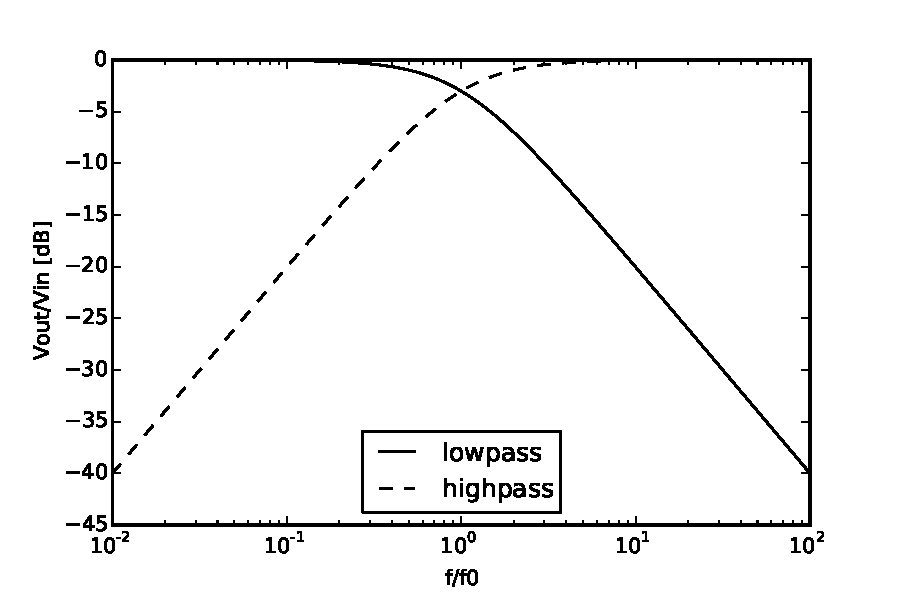
\includegraphics[height=0.22\textheight]{figs/bode.pdf}
&
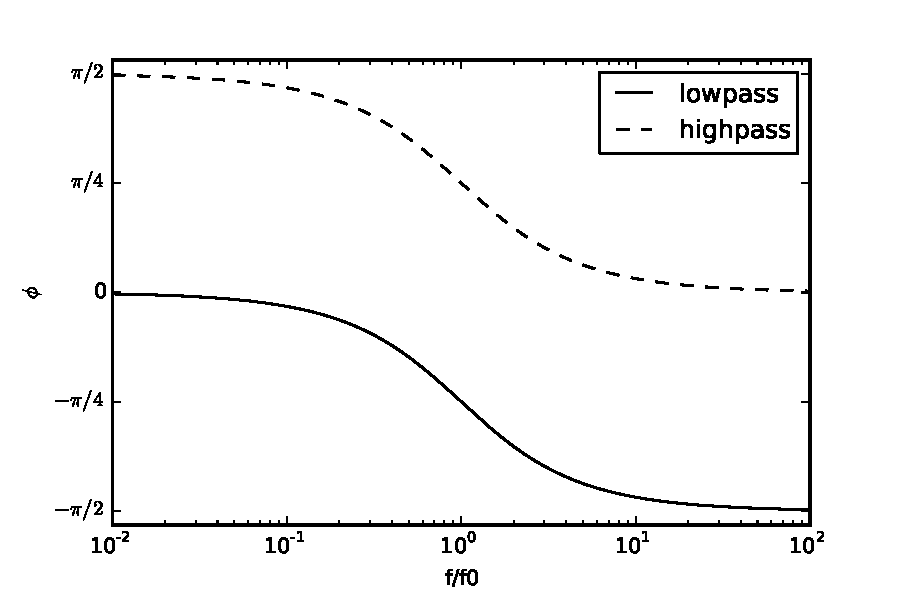
\includegraphics[height=0.22\textheight]{figs/phase.pdf} \\
(a) & (b) \\
\end{tabular}
\end{center}
\caption{\label{fig:bode} Bode plots for highpass and lowpass filters showing the (a) gain on a dB scale, and (b) phase, both as a function of the ratio of frequency $f$ to the crossover frequency $f_0$ on a log scale.}
\end{figure}

In this lab, you will build and measure the performance of a lowpass and a highpass $RC$ filter, and produce Bode plots to compare your circuit with the impedance model derived in class and shown in Fig.~\ref{fig:bode}.  You will build an $RLC$ bandpass filter, determine its resonant frequency and quality factor, and see how limitations from non-ideal components dramatically affect the performance of real circuits.

\section{Lowpass Filters}

\begin{figure}[htbp]
\begin{center}
\begin{tabular}{c@{\hskip 1in}c}
\begin{picture}(110,130)
\put(0,0){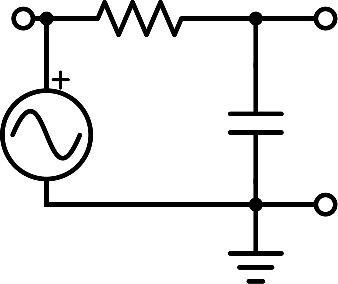
\includegraphics[height=0.15\textheight]{figs/rc.pdf}} 
\put(-12,98){$V_{\rm in}$}
\put(-6,70){$\widetilde{V}$}
\put(72,55){$C$}
\put(50,80){$R$}
\put(114,38){$P_{1}$}
\put(114,82){$V_{\rm out}$}
\end{picture}
&
\begin{picture}(140,130)
\put(0,0){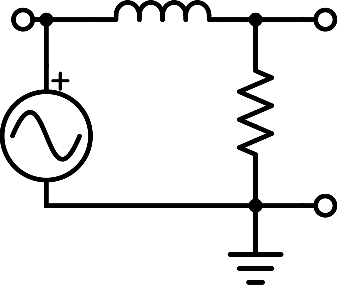
\includegraphics[height=0.15\textheight]{figs/lr.pdf}}
\put(-12,98){$V_{\rm in}$}
\put(-6,70){$\widetilde{V}$}
\put(72,55){$R$}
\put(50,85){$L$}
\put(114,38){$P_{1}$}
\put(114,82){$V_{\rm out}$}
\end{picture}\\
(a) & (b) \\
\end{tabular}
\end{center}
\caption{\label{fig:lowpass} Circuit diagrams for lowpass filters featuring (a) a capacitor, and (b) an inductor.}
\end{figure}

\noindent
You'll be using two scope probes in this lab, and some care must be taken when using their grounding clips.  The only place you may connect the grounding clip from a scope probe is to the ground in your circuit. For a battery powered device not connected to earth ground, you could choose this ground point to be anywhere, as long as it was consistent for both scope channels.  But in our circuit, the function generator is already referenced to earth ground, and therefore the only possible choice for the ground location is at the negative terminal of the function generator, as already shown in the circuit diagrams.  Always remember that when you connect a scope probe grounding clip, you short that point to earth ground through the scope!  {\bf In these circuits, the only place you may attach a scope probe grounding clip is at the point $\boldmath P_1$, i.e. at the negative terminal of the function generator.}


\begin{figure}[htbp]
\begin{center}
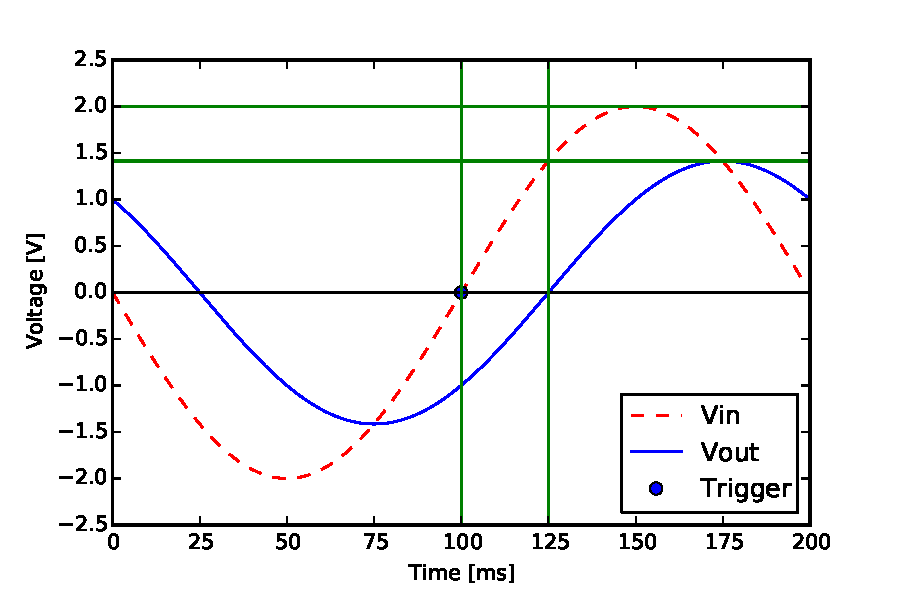
\includegraphics[height=0.35\textheight]{figs/scope_gain.pdf}
\end{center}
\caption{\label{fig:scopegain} The gain and phase change measurement using an oscilloscope.
Here the gain is $1.4/2.0 = 0.7 \sim 1/\sqrt{2}$.  Later times appear toward the right, so the output is lagging the input, and therefore the phase shift is negative.  The size of the time offset is $25~\rm ms$ in a period of $200~\rm ms$ so the phase shift is $\phi = -\pi/4$.  This is what engineers like to call the $-3~\rm dB$ or even just the $3~\rm dB$ point, because $20 \log_{10} \sqrt{2} = 3.01$.  Just to confuse physicists!}
\end{figure}

We'll be measuring two potentials simultaneously for all of the filters in this lab.  The input voltage $V_{\rm in}$ is measured between ground at $P_1$ and the point $V_{\rm in}$ in the circuit.  This can be measured by using a ``BNC T" to connect both your scope and your circuit to the function generator output.  Alternatively, use a scope probe with the grounding clip at $P_1$ and the the probe tip at $V_{\rm in}$.  The output voltage $V_{\rm out}$ is measured using a scope probe with the grounding clip at $P_1$ and the probe tip at $V_{\rm out}$.  We will be measuring the voltage gain $G = V_{\rm out} / V_{\rm in}$ and the phase shift $\phi$ of $V_{\rm out}(t)$ relative to $V_{\rm in}(t)$. 

Build the circuit shown in Fig.~\ref{fig:lowpass}a using $R=1.5~\rm k \Omega$ and $C= 0.01~\rm \mu F$.   Use your function generator in AC mode with a peak-to-peak voltage of $4~\rm V$.   Either put the function generator in high impedance output mode, or select the $50~\rm \Omega$ output impedance and use a $50~\rm \Omega$ terminator.

Vary the frequency above and below the cross-over frequency which you calculated, and verify the behavior qualitatively before proceeding with the data taking.  As this is a low-pass filter, you should expect to see the gain $V_{\rm out}/V_{\rm in} = 1/\sqrt{2}$ with a phase shift $\phi = -\pi/4$ at the crossover frequency.  An example measurement at the crossover frequency is shown in Fig.~\ref{fig:scopegain}.  Below this frequency you should approach unit gain, and above this frequency the gain should fall rapidly.  

To make these measurements accurately, you should first confirm that both channel 1 and channel 2 on your scope are vertically aligned with the $x$-axis (i.e. the thick central horizontal line on the display), which you do by temporarily setting the coupling of each channel to ground (i.e. V=0) and adjusting the horizontal offset as needed.  Next, adjust the trigger setting to trigger on the rising edge of $V_{\rm in}$ and set the trigger threshold at zero.  Learn to use your scope's cursor function.  For instance, when making the phase shift measurement, you would place the reference cursor at the point where 
$V_{\rm in}$ crosses zero with positive slope (the trigger point) and measure the point where $V_{\rm out}$ crosses zero with positive slope using the cursor.

Once you are certain your circuit is working properly and you scope is configured to measure the magnitude and gain accurately, take measurements at 9 different frequencies, chosen to cover four decades of frequency range and uniform in the log of the frequency:
\begin{displaymath}
f=\{f_0/100, f_0/30, f_0/10, f_0/3,f_0, 3f_0, 10f_0, 30f_0, 100f_0\}
\end{displaymath}
where $f_0$ is the cross-over frequency.  At each frequency, you will measure the gain:  $G = V_{\rm out} / V_{\rm in}$ and the phase shift $\phi$ of $V_{\rm out}$ relative to $V_{\rm in}$.  

If you prefer, you can use your scope's measurement features (which include a phase measurement) after making a few measurements from the wave form as described above.  When using automated features, it is usually a good idea to make a few manual measurements first to make sure you are measuring what you think you are.

\section{Highpass Filter}

\begin{figure}[htbp]
\begin{center}
\begin{tabular}{c@{\hskip 1in}c}
\begin{picture}(110,130)
\put(0,0){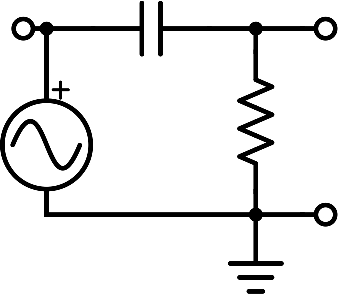
\includegraphics[height=0.15\textheight]{figs/cr.pdf}} 
\put(-12,98){$V_{\rm in}$}
\put(-6,70){$\widetilde{V}$}
\put(72,55){$R$}
\put(50,70){$C$}
\put(114,38){$P_{1}$}
\put(114,82){$V_{\rm out}$}
\end{picture}
&
\begin{picture}(140,130)
\put(0,0){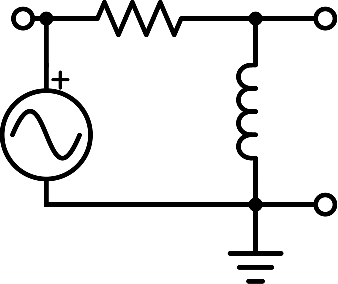
\includegraphics[height=0.15\textheight]{figs/rl.pdf}}
\put(-12,98){$V_{\rm in}$}
\put(-6,70){$\widetilde{V}$}
\put(75,55){$L$}
\put(50,78){$R$}
\put(114,38){$P_{1}$}
\put(114,82){$V_{\rm out}$}
\end{picture}\\
(a) & (b) \\
\end{tabular}
\end{center}
\caption{\label{fig:highpass} Circuit diagrams for highpass filters featuring (a) a capacitor, and (b) an inductor.}
\end{figure}

Using the same components as in the previous section, build the high-pass filter of Fig.~\ref{fig:highpass}a.  Verify the operation of the circuit at the crossover frequency (aka 3 db point) where we expect the gain to be $1/\sqrt{2}$ as before but the phase shift to be {\em positive} $\phi = \pi/4$.

As in the preceding section, measure the magnitude and phase of the gain as a function of frequency, but to save time, you may omit some measurements:
\begin{displaymath}
f=\{f_0/10, f_0/3,f_0, 3f_0, 10f_0\}
\end{displaymath}
where $f_0$ is the crossover frequency.

\section{Bandpass Filter}

\begin{figure}[htbp]
\begin{center}
\begin{picture}(230,100)
\put(0,0){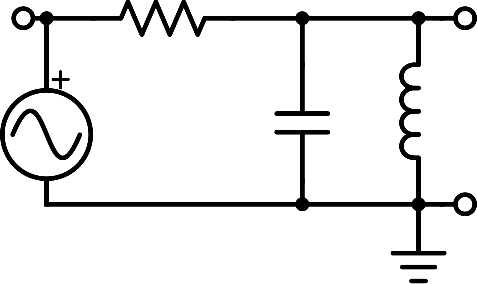
\includegraphics[height=0.15\textheight]{figs/rlc.pdf}} 
\put(-12,98){$V_{\rm in}$}
\put(-6,70){$\widetilde{V}$}
\put(60,80){$R$}
\put(120,68){$C$}
\put(135,45){$L$}
\put(170,42){$P_{1}$}
\put(170,78){$V_{\rm out}$}
\end{picture}
\end{center}
\caption{\label{fig:rlc} Circuit diagram for an RLC band-pass filter, with $Q$-spoiling resistor $R_2$.}
\end{figure}

In lecture, we showed that the resonant angular frequency of an RLC bandpass filter is given by
\begin{equation}
\omega_0 = \frac{1}{\sqrt{LC}}. 
\end{equation}
At this frequency, the RLC resonant circuit has unit gain and no phase shift.  As the frequency moves away from the resonant frequency, the gain drops.  We define two points $\omega_+$ and $\omega_-$ as the two frequencies, one above and one below $\omega_0$, at which the gain drops below $1/\sqrt{2}$.  These are the two $-3~\rm dB$ points which define the bandwidth of the system.  We define the quality of the resonance by the ratio of resonant frequency to this bandwidth:
\begin{displaymath}
Q = \frac{\omega_0}{\omega_+ - \omega_-} = \frac{f_0}{f_+-f_-}
\end{displaymath}
For the RLC resonant circuit, we showed in lecture that:
\begin{equation}
Q = \omega_0 RC
\end{equation}

Build the circuit in Fig.~\ref{fig:rlc} using $R=1~{\rm k \Omega}$ , $C=4.7~\rm{\mu F}$, and $L=150~\rm \mu H$.
Set the frequency of the function generator to $f_0 = \omega_0/2\pi$  and the peak-to-peak voltage $10~\rm V$.

\begin{figure}[htbp]
\begin{center}
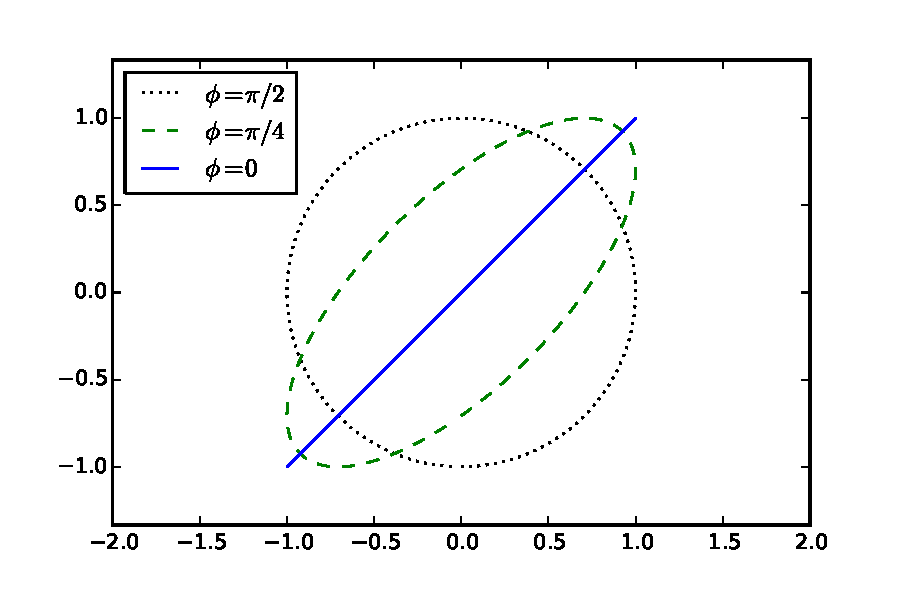
\includegraphics[height=0.35\textheight]{figs/scope_xy.pdf}
\end{center}
\caption{\label{fig:scopexy} Example scope traces in XY display mode for a relative phase $\phi=\pi/2$, 
$\phi=\pi/4$, and $\phi=0$.  It is easy, accurate, and somehow deeply satisfying to tune the frequency until the ellipse collapses into itself, forming a line.}
\end{figure}

We'll determine the resonant frequency using a trick.  During normal use, your oscilloscope displays the voltage of each channel versus time.  But there is an ``XY" mode available under the display options.  In this mode, the scope displays the voltage of channel one versus the voltage of channel two.  When in XY mode, two out-of-phase signals yield an ellipse.  But, as shown in Fig.~\ref{fig:scopexy} when both channels are perfectly in phase, the ellipse collapses to make a diagonal line.  You can set you scope in XY mode and adjust the frequency until the ellipse collapses to quickly and accurately find the resonance frequency.

One you determine the resonant frequency, switch back to the normal display mode and determine the bandwidth.  The easiest way to obtain this is to use the curser to measure the peak voltage of your output signal.  Multiply this by a factor of $1/\sqrt{2} = 0.7$ to determine the $-3~\rm dB$ amplitude and set the second curser at this value.  Now adjust the frequency above and below the resonant frequency and note at which frequencies the amplitude drops below this line.  The difference between these two points is your $f_+$ and $f_-$.

From your measurement of $f_0$, $f_+$, and $f_-$ you can calculate the measured $Q$-factor of your circuit.  It will be quite different than what you calculated in pre-lab! 

\section{Degradation of the $Q$-factor}

The $Q$-factor that you measured in the previous section is significantly lower than the theoretical $Q$-factor for the circuit in Fig.~\ref{fig:rlc}.  In fact, the inductor is non-ideal in a number of ways.  In this case, there is a parasitic parallel resistance that makes the circuit effectively that of Fig.~\ref{fig:rlcpar}.  The resistance $R_{\rm P}$ is already present (unfortunately!) in your circuit.  

It turns out that the $Q$ factor is degraded in this case to the value:
\begin{equation}
Q = \omega_0 C \frac{R R_{\rm P}}{R+R_{\rm P}}
\end{equation}

To determine $R_P$, note that at the resonant frequency, the parallel impedance of $L$ and $C$ are infinite, and so can be treated as open circuits.  The circuit becomes a voltage divider with two resistors $R$ and $R_P$.  By measuring the gain $V_{\rm out}/V_{\rm in}$ at the resonant frequency, you should be able to determine $R_P$, and correct your gain calculation accordingly.  Now how does your calculated $Q$-factor compare with what you measured?

\begin{figure}[htbp]
\begin{center}
\begin{picture}(230,100)
\put(0,0){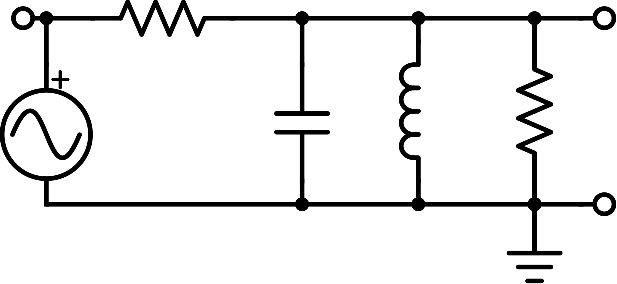
\includegraphics[height=0.15\textheight]{figs/rlcpar.pdf}} 
\put(-12,98){$V_{\rm in}$}
\put(-6,70){$\widetilde{V}$}
\put(60,80){$R$}
\put(120,68){$C$}
\put(155,45){$L$}
\put(170,65){$R_{\rm P}$}
\put(220,42){$P_{1}$}
\put(220,78){$V_{\rm out}$}
\end{picture}
\end{center}
\caption{\label{fig:rlcpar} Circuit diagram for an RLC band-pass filter, with $Q$-spoiling parasitic parallel resistance $R_{\rm P}$.}
\end{figure}

\section{Lab Report}

Your report should include all of your calculations, and the plotted response of your lowpass and highpass circuits as in Fig.~\ref{fig:bode}.  In addition to the gain in dB, also produce a plot with $V_{\rm out}/V_{\rm in}$.  Answer all questions in the text.

Notice that the difference between the RC highpass and lowpass filter just amounts to which component we measure the voltage $V_{\rm out}$ across.  Therefore, one might reasonably expect the crossing point of the Bode plots to occur where $V_{\rm out}/V_{\rm in} = 0.5$, but, in fact, it occurs at the 3~dB point where $V_{\rm out}/V_{\rm in} = 0.7$.  How is this be possible?  Does the voltage across the resistor plus the voltage across the capacitor add to 1.4 times the input voltage?!

 
\end{document}
